
\documentclass[oneside]{diretrizes}            % Imprimir apenas frente
%\documentclass[doubleside]{diretrizes}        % Imprimir frente e verso

% Importações de pacotes
\usepackage[alf, abnt-emphasize=bf, recuo=0cm, abnt-etal-cite=2, abnt-etal-list=0]{abntex2cite}  % Citações padrão ABNT
\usepackage[utf8]{inputenc}                         % Acentuação direta
\usepackage[T1]{fontenc}                            % Codificação da fonte em 8 bits
\usepackage{graphicx}                               % Inserir figuras
\usepackage{amsfonts, amssymb, amsmath}             % Fonte e símbolos matemáticos
\usepackage{booktabs}                               % Comandos para tabelas
\usepackage{verbatim}                               % Texto é interpretado como escrito no documento
\usepackage{multirow, array}                        % Múltiplas linhas e colunas em tabelas
\usepackage{indentfirst}                            % Endenta o primeiro parágrafo de cada seção.
\usepackage{microtype}                              % Para melhorias de justificação?
\usepackage[algoruled, portuguese]{algorithm2e}     % Escrever algoritmos
\usepackage{float}                                  % Utilizado para criação de floats
\usepackage{times}                                  % Usa a fonte Times

% Inclui o preâmbulo do documento
%
% Documento: Preâmbulo
%

\instituicao{Instituto Federal de Educação, Ciência e Tecnologia \\do Rio Grande do Sul}
\abreviatura{IFRS}
\departamento{Campus Restinga}
\local{Porto Alegre}
\programa{Análise e Desenvolvimento de Sistemas}
\nomeautor{Felipe dos Santos Viegas}
\titulotb{Pybot}
%\subtitulo{Subtítulo do trabalho}
\data{2017}
\grau{Tecnólogo}
\dataapresentacao{DD/MM/20AA}

%Dados Orientador
\orientador{Roben Castagna Lunardi}
%\coorientador{Anderson Black}
\instOrientador{IFRS}
\departamentoorientador{Campus Restinga}
\titulacaoorientador{Prof. Me.}

%Dados Coorientador
%\coorientador{Artur Dent}
%\instCoorientador{IFRS}
%\departamentocoorientador{Campus Restinga}
%\titulacaocoorientador{Prof. Dr.}

%Dados Examinador 1
\nmexamum{Mestre dos Magos}
\instexamum{IFRS}
\departamentoexamum{Campus Restinga}
\titulacaoexamum{Prof.}

%Dados Examinador 2
\nomeexamdois{Mestre Splinter}
\instexamdois{IFRS}
\departamentoexamdois{Campus Restinga}
\titulacaoexamdois{Prof. Me.}


% Define as cores dos links e informações do PDF
\makeatletter
\hypersetup{
    portuguese,
    colorlinks,
    linkcolor=black,
    citecolor=black,
    filecolor=black,
    urlcolor=black,
    breaklinks=true,
    pdftitle={\@title},
    pdfauthor={\@author},
    pdfsubject={\imprimirpreambulo},
    hypertexnames=false,
    pdfkeywords={abnt, latex, abntex, abntex2}
}
\makeatother

% Redefinição de labels
\renewcommand{\algorithmautorefname}{Algoritmo}
\def\equationautorefname~#1\null{Equa\c c\~ao~(#1)\null}

% Cria o índice remissivo
\makeindex

% Início do documento
\begin{document}

    % Retira espaço extra obsoleto entre as frases.
    \frenchspacing

    % Elementos pré textuais
    \pretextual
    %
% Documento: Capa
%

\makeatletter
\begin{capa}
	\thispagestyle{empty}%limpa estilo da pagina
	\setlength{\baselineskip}{0.72\baselineskip}
    \begin{center} %Alinhamento centralizado
	

    \textbf{\expandafter\uppercase\expandafter{\imprimirinstituicao}}\\
    \textbf{\expandafter\uppercase\expandafter{\imprimirdepartamento}}\\
    \textbf{\expandafter\uppercase\expandafter{\imprimirprograma}}\\
	\vspace*{5cm}%Espaçamento entre linhas
	\large\textbf{\expandafter\uppercase\expandafter{\imprimirtitulotb}}\\
	\vspace*{6cm}%Espaçamento entre linhas	
	\small\textbf{\expandafter\uppercase\expandafter{\imprimirnomeautor}}\\
	\vspace*{9.5cm}%%Espaçamento entre linhas
	\small\textbf{\expandafter\uppercase\expandafter{\imprimirlocal}}\\
	\small\textbf{\expandafter\uppercase\expandafter{\imprimirdata}}\\
		
		
		
	\end{center} %Alinhamento centralizado
\end{capa}
\makeatother

	

              % Capa
    %
% Documento: FOLHA DE ROSTO
%

\makeatletter
\begin{folhaderosto}
	\thispagestyle{empty}%limpa estilo da pagina
	
    \begin{center}
    
		\small\textbf{\expandafter\uppercase\expandafter{\imprimirnomeautor}}\\
		\vspace*{8.2 cm}%Espaço entre linhas
		\normalsize\textbf{\expandafter\uppercase\expandafter{\imprimirtitulotb}}\\
		
    \end{center}
	
	\vspace*{0.35 cm}%Espaçamento entre linhas
		    \large%tamanho da fonte 
    		\hfill%Estica horizontamente  com espaços
	    	\begin{minipage}{8 cm}%Minipagina
	    		\begin{small} %Muda tamanho da fonte
	    		\setlength{\baselineskip}{0.7\baselineskip}
				
		    	{Trabalho de Conclusão de Curso apresentada como requisito parcial para obtenção do grau de
		    	{\imprimirgrau } em {\imprimirprograma } da {\imprimirinstituicao}{ - }{\imprimirabreviatura},
		    	{\imprimirdepartamento}.}\\{
		    	}\\Orientador: {\imprimirtitulacaoorientador }{ }{\imprimirorientador}\\{
		    	}\\Co-orientador: {\imprimirtitulacaocoorientador }{ }{\imprimircoorientador}
				
				
				\end{small} %Muda tamanho da fonte
		    \end{minipage}%%Minipagina
		    	
		    \vspace*{10 cm}%Espaçamento entre linhas
		    
		    \begin{center} %Alinhamento centralizado
		    	\normalsize %Muda tamanho da fonte
	    		\imprimirlocal\\
	    		\imprimirdata
	    	\end{center}%Alinhamento centralizado

\end{folhaderosto}
\makeatother
        % Folha de rosto
    %
% Documento: FOLHA APROVAÇÃO
%

\makeatletter
\begin{folhadeaprovacao}

\thispagestyle{empty}%limpa estilo da pagina
	
	\begin{center}
    
		\small\textbf{\expandafter\uppercase\expandafter{\imprimirnomeautor}}\\
		\vspace*{3.0 cm}%Espaço entre linhas
		\normalsize\textbf{\expandafter\uppercase\expandafter{\imprimirtitulotb}}
		
    \end{center}
	
	\vspace*{0.35 cm}%Espaçamento entre linhas
		    \large%tamanho da fonte 
    		\hfill%Estica horizontamente  com espaços
	    	\begin{minipage}{8 cm}%Minipagina
	    		\begin{small} %Muda tamanho da fonte
	    		\setlength{\baselineskip}{0.7\baselineskip}
				
		    	{Trabalho de Conclusão de Curso apresentado como requisito parcial para obtenção do grau de
		    	{\imprimirgrau } em {\imprimirprograma } do {\imprimirinstituicao}{ - }{\imprimirabreviatura},
		    	{\imprimirdepartamento}.}\\{
		    	}\\				
				
				\end{small} %Muda tamanho da fonte
		    \end{minipage}%%Minipagina
		    	
		    \vspace*{0.6 cm}%Espaçamento entre linhas
		    
		    \large%%tamanho da fonte 
    		\hfill%%Estica horizontamente  com espaços
	    	 
		    
		    \normalsize %Muda tamanho da fonte
		    \vspace*{1.5 cm}%Espaçamento entre linhas
		    
		    \begin{minipage}{9 cm }%%Minipagina
		    {Data de Aprovação: {\imprimirdataapresentacao}}\\
		    \end{minipage}%Minipagina
			
			\begin{center}%Alinhamento centralizado
		    	\vspace*{1.21 cm}%Espaçamento entre linhas
				\textbf{Banca Examinadora}\\ %Negrito
						
				\vspace*{1 cm}%Espaçamento entre linhas
				\rule{9 cm}{.1 mm}\\
				{\imprimirtitulacaoorientador}{ }{\imprimirorientador} - {\imprimirinstOrientador} - {\imprimirdepartamentoorientador}\\
				Orientador\\
				
				\vspace*{1 cm}%Espaçamento entre linhas
				\rule{9 cm}{.1 mm}\\
				\imprimirtitulacaoexamum{ }\imprimirnmexamum - \imprimirinstexamum - \imprimirdepartamentoexamum\\
				Membro da Banca
				
				\vspace*{1 cm}%Espaçamento entre linhas
				\rule{9 cm}{.1 mm}\\				
								
				\imprimirtitulacaoexamdois{ }\imprimirnomeexamdois - \imprimirinstexamdois - \imprimirdepartamentoexamdois\\
				Membro da Banca
				\vspace*{1.3 cm}%Espaçamento entre linhas
		    \end{center}%Alinhamento centralizado


\end{folhadeaprovacao}
\makeatother
    % Folha de aprovação
    %
% Documento: Folha Catalográfica
%

\thispagestyle{empty}
\vspace*{\fill}

 \begin{flushleft}
\small \setlength{\baselineskip}{0.8\baselineskip}INSTITUTO FEDERAL DE EDUCAÇÃO, CIÊNCIA E TECNOLOGIA DO RIO GRANDE DO SUL\\
Reitor: Prof. Osvaldo Casares Pinto\\
Pró-Reitora de Ensino: Profa. Clarice Monteiro Escott\\
Diretor do Campus Restinga: Prof. Gleison Samuel do Nascimento\\
Coordenador do Curso de Ciência da Computação: Prof. Rafael Pereira Esteves\\
Bibliotecária-Chefe do Campus Restinga: Paula Porto Pedone\\
\end{flushleft}



    %
% Documento: Dedicatória
%

\thispagestyle{empty}
\begin{dedicatoria}

Dedico esse trabalho a todos aqueles que me ajudaram do fim ao começo!

\end{dedicatoria}
       % Dedicatória
    % %
% Documento: Agradecimento
%

\begin{agradecimento}

Neste trecho você faz agradecimentos dirigidos aqueles que contribuíram de maneira relevante a elaboração do trabalho.
Elemento opcional segundo a norma da ABNT NBR 14724 de 2011.

\end{agradecimento}

    % Agradecimentos
    % %
% Documento: Epígrafe
%
\thispagestyle{empty}
\begin{epigrafe}


O fator decisivo para vencer o maior obstáculo é, invariavelmente, ultrapassar o obstáculo anterior.{\\}{\\}

\begin{autorepigrafe}
Henry Ford
\end{autorepigrafe}

\end{epigrafe}


          % Epígrafe
    %
% Documento: Resumo (Português)
%

\begin{RESUMO}
\thispagestyle{empty}
	\begin{SingleSpace}


		Em muitas empresas temos uma certa carência quando o assunto é automação de testes ou processos web em navegadores. A necessidade de testes de regressão, testes de funcionalidades e ou
        automação de processos cresce junto com o sistema, porem a pratica dessas atividades só tem força quando aparece aguma necessidade ou problema.

        Esse novo framework pretende trazer aos usuarios uma ferramenta de facil uso e com recursos uteis para o desenvolvimento dessas tarefas, contando com a facilidade e versatilidade da
        linguagem python e a integração com navegadores com framework selenium.

        O conjuntos de ferarmentas que o framework dispõe são: gerenciamento automatico dos controladores de navegadores(drivers), modulo de relatorios e logs para controle de atividades executadas,
        padronização de criação de elementos de tela utilizando o padrão PageObject.

		\vspace*{0.5cm}\hspace{-1.3 cm}\textbf{Palavras-chave}: Automação, Selenium, Testes.

	\end{SingleSpace}
\end{RESUMO}


          % Resumo na língua vernácula
    %
% Documento: Resumo (Inglês)
%

\begin{ABSTRACT}
	\begin{SingleSpace}


        Currently, many companies lack a solution for  test automation or web process management integrated to the browsers.
        The need for regression testing, functionality testing, and / or process automation grows along with the system,
        but the practice of these activities is only emerge when a need or problem appears.

        In order to solve this problem, we propose a framework aims to present to  users an easy-to-use tool with useful resources for the development of these
        tasks, with the simplicity and versatility of the \textit{Python} language and the integration with browsers with \textit{selenium framework}.

        The sets of tools that the proposed framework presents are: automatic management of the drivers of navigators (\textit{drivers}); module containing reports
        and logs to control activities performed; standardization of screen elements development using the standard \textit{PageObject} and identification of layout change.

		\vspace*{0.5cm}\hspace{-1.3 cm}\textbf{Palavras-chave}: Automation, Selenium, Tests.


	\end{SingleSpace}

\end{ABSTRACT}
          % Resumo em língua estrangeira
    %
% Documento: Lista de figuras
%

\pdfbookmark[0]{\listfigurename}{lof}
\listoffigures*
\cleardoublepage

      % Lista de figuras
    % %
% Documento: Lista de tabelas
%

\pdfbookmark[0]{\listtablename}{lot}
\listoftables*
\cleardoublepage
      % Lista de tabelas
    % %
% Documento: Lista de quadros
%

\pdfbookmark[0]{\listofquadrosname}{loq}
\listofquadros*
\cleardoublepage
      % Lista de quadros
    % %
% Documento: Lista de abreviaturas e siglas
%

\begin{siglas}
	\setlength{\baselineskip}{0.7\baselineskip}
	
    \item[ABNT] Associação Brasileira de Normas Técnicas
    \item[TCC] Trabalho de Conclusão do Curso
    \item[NBR] Norma Brasileira
\end{siglas}
       % Lista de abreviaturas e siglas
    %%
% Documento: Lista de símbolos
%

\begin{simbolos}
    \item[$ \Gamma $] Letra grega Gama
    \item[$ \lambda $] Comprimento de ondada
    \item[$ \in $] Pertence
\end{simbolos}
     % Lista de símbolos
    \sumario

    % Elementos textuais
    \textual
    %
% Documento: Introdução
%

\chapter{INTRODUÇÃO}\label{chap:introducao}

O ciclo de vida de software tem diveras etapas, de um modo geral elas são: Análise de requisitos, Concepção do Projeto, Desenvolvimento, Implantação e por fim Manutenção.
Nas etapas de Desenvolvimento e a Manutenção é onde a criação ou a codificação do software em questão mais acontece, e na concepção de um projeto a necessidade da criação
de um processo de testes que cresça junto do sistema não tem a sua devida importação.


Este Trabalho de Conclusão de Curso tem como objetivo criar um framework para auxiliar nas tarefas de criação de testes e ou automatização de processos de sistemas executados em navegadores.
Levando o nome de PyBot, união das palavras Python, liguagem utilizada para criação do projeto, e Bot, que em inglês quer dizer robô, essa ferramenta propõe prover para os usuarios uma serie
de ferramentas para auxiliar a criação e implantação desses processos, contando uma estrutura de criação dos scripts de teste no padrão PageObject e PageElement, geração de registros de logs
para controle de tarefas e passos executados, verificação de alteração de interfaces e layout dos sites e o gerenciamento automatico de drivers de navegadores com a ferramenta Driloader.            % Introdução
    %
% Documento: Disposições
%

\chapter{Framework Proposto}

    Neste capítulo irei abordar as tecnologias de utilizadas para a codificação do framework,
    detalhando os módulos e suas classes expostas para o usuário e as ferramentas utilizadas
    para controle de versão e publicação do framework.


    \section{Tecnologias Utilizadas}

        Para o desenvolvimento do framework foi utilizado apenas como linguagem para desenvolvimento o Python
        e para a manipulação e integração com o \emph{browser} a biblioteca em Python do Selenium \emph{Webdriver}. Por ser um
        projeto que visa ser o mais simples e leve possível apenas os módulos padrões do Python estão sendo utilizado
        para o desenvolvimento desta ferramenta.


        \subsection{Python}

            A escolha do Python \cite{Python} foi devida porque ele trata-se de uma linguagem de programação fácil de aprender e poderosa.
            Possuindo uma estruturas dados de alto nível e uma abordagem simples, mas eficaz, para a programação orientada
            a objetos. Contendo uma Sintaxe elegante e tipagem dinâmica, juntamente com uma interpretação natural, tornam
            a linguagem ideal para criação dos \emph{scripts} do Pybot.

        \subsection{Selenium WebDriver}
            \emph{Selenium Webdriver} \cite{webdriver} é um framework utilizado para se comunicar e enviar comandos para os \emph{browser}
            em conjunto com um controlador de cada \emph{browser} específico. Em comparação com seu antecessor, Selenium RC, o Selenium \emph{Webdriver}
            não precisa de um server para enviar os comandos para o \emph{browser}. Utilizando comando nativos do sistema operacional ao invés de
            comando javascript, usados pelo Selenium RC, deixam o Selenium \emph{Webdriver} uma excelente ferramenta para integração com diversos
            \emph{browser}.

        \subsection{Git e GitHub}
            Para o controle de versões e alterações do código fonte do framework e \emph{scripts} de exemplo foi utilizado a ferramenta
            Git \cite{git} em conjunto com os servidores do Github \cite{github} para hospedagem e gerenciamento. Com eles foi possível
            fazer alterações dos códigos fontes em qualquer computador e gerenciar os erros e melhorias do framework.


    \section{Módulos}

        O framework consiste em alguns módulos básicos, cada um com suas devidas utilidades e funções.
        A separação dos de cada módulos foi dada com base em suas caracteristicas e funcionalidades,

        \begin{figure}[H]
            \vspace*{0,3cm}
            \centering
            \caption{Diagrama de Componentes}
            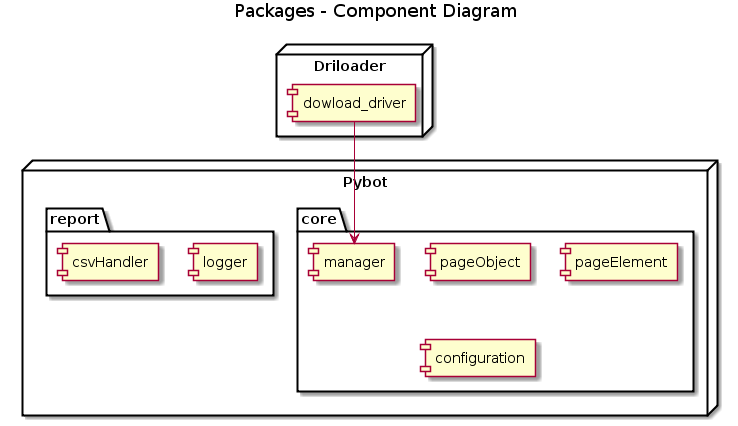
\includegraphics[width=1\textwidth]{./04-figuras/model}
            \label{fig:modules}
        \end{figure}

        \subsection{Core}
            Este módulo contém as funcionalidades básicas para a operação do framework com o Selenium \emph{Webdriver}
            e o gerenciamento dos parâmetros de execuções de cada script.

            \subsubsection{Manager}
            Manager server para abstrair o uso do Selenium \emph{Webdriver} criando uma camada de metodos própios fazendo com que caso alguma
            atualização da API do Selenium \emph{Webdriver} altere os \emph{scripts} criados não sejam impactados. Fazendo uso do Driloader mencionado na
            subseção \ref{driloader} ele verifica a necessidade do download do driver para poder executar o \emph{Selenium Webdriver}.

            \subsubsection{Configuration}
            Responsável por gerar as configurações básicas para o framework e disponibilizá-las no arquivo \emph{pybot.ini}.
            Este arquivo é criado para cada script do usuário e nele arquivo é possível adicionar qualquer tipo de configurações ou parâmetros
            necessárias para o usuário, apenas sendo preciso seguir os padrões descrito na imagem \ref{fig:pybot.ini} e utilizando com o comando
            \mbox{\emph{configuration.getConfig('Seção', 'variável')}}

            \begin{figure}[H]
                \vspace*{0,3cm}
                \centering
                \caption{Estrutura pybot.ini}
                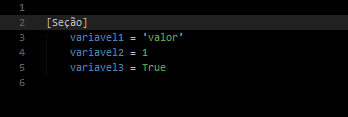
\includegraphics[width=0.7\textwidth]{./04-figuras/ini}
                \label{fig:pybot.ini}
            \end{figure}

        \subsection{Component}
        \label{Comp}
            Módulo criado para seguir os padrões de \emph{PageObject} e \emph{PageElement}, contendo abstração para os tipos de inputs do \emph{html}.

            \subsubsection{WebElement}
                Serve para abstrair o uso da classe WebElement do próprio Selenium Webdriver. Contendo uma classe para cada tipo de campo dos \emph{html},
                ele dispõe de algumas funcionalidades básica, como a atribuição de uma valor para um elemento do tipo \emph{input text} irá escrever
                valor dentro do campo, \emph{select} irá selecionar a opção cujo texto seja igual ao valor informado, \emph{radio} irá selecionar o
                a opção que tenha o \emph{value} do valor informado e para o tipo \emph{checkbox} irá marcar ou desmarcar as opções se o valor for
                verdadeiro(True) ou falso(False)

            \subsubsection{PageElement e PageElements}
            \label{PageElement}
                Essas classes servem para controlar os elementos mapeados das telas. Sempre quando serão acessadas a classe faz novamente a pesquisa
                do elemento em tela, prevenindo assim uma das exceções mais comum do Selenium Webdriver que é a \emph{StaleElementReferenceException},
                que é quando o elemento em questão não existe mais no DOM ou a referência que tinha não é mais a mesma. Conta com uma lista de seletores
                que facilitam para o usuário buscar os elementos e deixam o código mais legível. Usa-se a classe PageElements quando quiser pegar mais
                de um elemento com o mesmo seletor.

                \begin{figure}[H]
                    \vspace*{0,3cm}
                    \centering
                    \caption{Lista de Seletores}
                    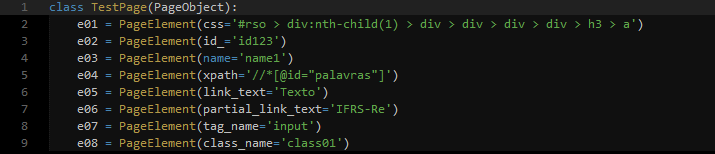
\includegraphics[width=1\textwidth]{./04-figuras/selectors}
                    \label{fig:selectors.png}
                \end{figure}

            \subsubsection{PageObject}
                Classe simbolica, serve apenas para poder juntar diversos PageElement descritos pelo usuário em uma classe para melhor
                legibilidade e componentização das páginas mapeadas.

        \subsection{Report}

            Estes módulo está destinado para geração de logs de execuções internas do framework, criação e controle
            de logs definidos pelos usuário e a criação de planilhas analíticas de dados extraídos das páginas.

            \subsubsection{Logger}
            Classe de geração dos Logs de execução do framework.

            \subsubsection{CsvHandler}
            Utilizado para geração de planilhas com dados extraídos das páginas para análise posterior do usuário.

        \subsection{Driloader}
        \label{driloader}
            Driloader é o responsavel pelo download dos driver de cada \emph{browser},suportando download dos driver do Internet Explorer,
            Firefox e Chrome, sendo possível para o usuário selecionar uma versão específica, a ultima versão ou detectar
            automaticamente qual a versão adequada para o \emph{browser} instalado do usuário. Como para utilização do Selenium
            Webdriver é necessário um driver específico de cada \emph{browser} foi tomada a decisão da criação desse projeto,
            inicialmente o Driloader era um módulo do framework mas pela autonomia e praticidade que ele proporciona aos
            usuários do Selenium Webdriver foi feita a separação dele do Pybot.



         % Implementação
    %
% Documento: Disposições
%

\chapter{Método de Desenvolvimento Proposto}\label{chap:proj}
    O framework proposto é baseado no conceito de PageObject, onde todas as páginas web são tratadas como objetos.
    Ainda, cada componente que seja necessário para automação, um \emph{input}, \emph{span}, etc, é um atributo desse objeto.

    Para melhor exemplificar o uso do conceito de PageObject será utilizado como exemplo um simples login para 2
    usuários, onde será utilizada uma página que possui dois campos de texto, campo de usuário e outro de senha,
    e um botão para submeter o login.

    Primeiro, utilizou-se um exemplo básico de como o \textit{Selenium} propõe o desenvolvimento mostrado na figura
    \ref{fig:selenium_default}. Primeiro é iniciado o \emph{driver} do navegador, navegar para a URL, depois
    são seguidos 3 passos para cada um dos campos de texto, procurar ele, limpar o conteúdo
    (porque não se sabe se ele possui algum texto pré cadastrado) e enviar os caracteres necessário para
    cada campo e por final, procurar e clicar no campo de submeter. Não é uma método muito viável, pois
    no caso temos 2 logins e o \emph{script} deverá ser duplicado para atender ambas necessidades.

    \begin{figure}[H]
        \vspace*{0,3cm}
        \centering
        \caption{Uso padrão Selenium}
        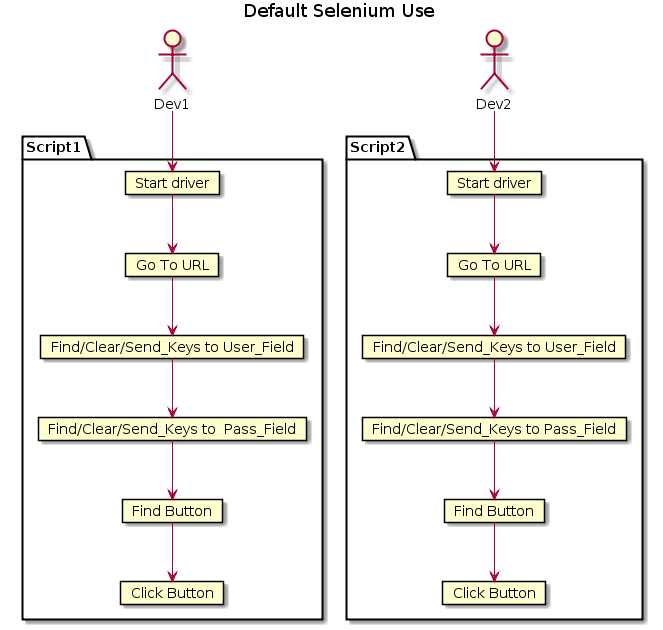
\includegraphics[width=0.8\textwidth]{./04-figuras/page_object_selenium}
        \label{fig:selenium_default}
    \end{figure}

    \clearpage

    Num segundo exemplo poderíamos separar o \emph{script} de login e criar um módulo separado para ele. Desse jeito
    os \emph{scripts} podem fazer uso do mesmo codigo e caso uma terceira pessoa precise dele não seria um problema.
    Porém temos todo o mapeamento dessa página preso num módulo e caso seja necessário a criação de outro
    módulo que use esses campos ainda assim teremos que duplicar mais codigo.

    \begin{figure}[H]
        \vspace*{0,3cm}
        \centering
        \caption{Uso padrão Selenium com módulo}
        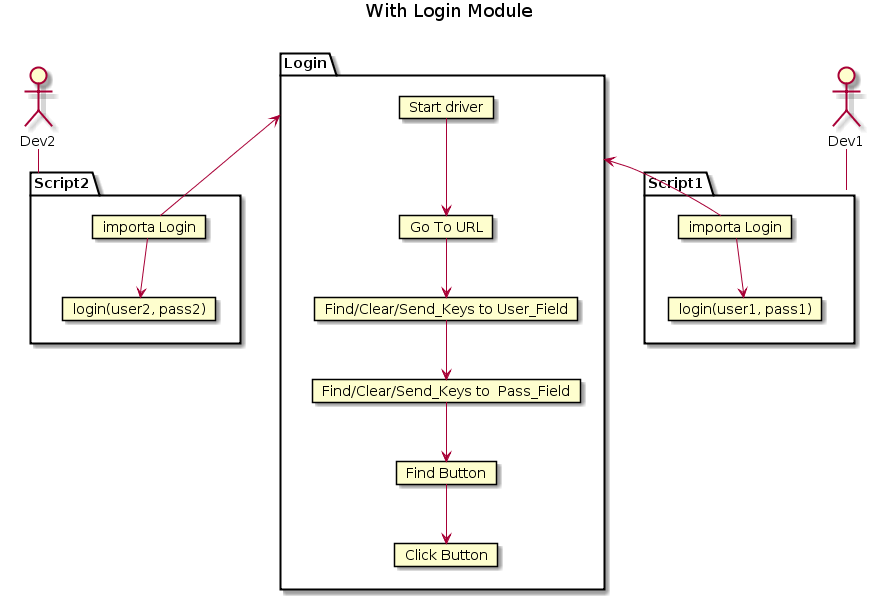
\includegraphics[width=1\textwidth]{./04-figuras/page_object_module}
        \label{fig:selenium_module}
    \end{figure}

    \clearpage
    Chegando num terceiro exemplo onde agora fazemos uso do framework \emph{Pybot}, onde utilizando-se do
    módulo Component(\ref{Comp}) podemos separar todos os componentes da tela em atributos da nossa página
    e criar um método onde precisando de dois parâmetros ele faz o processo de login, e ainda assim, caso
    necessário pode-se utilizar os campos mapeados para fazer algum outro método sem impactar o login.
    E caso alguma referencia dos campos mapeados mude, será necessário alterar apenas um local e nenhum \emph{script}
    será impactado.

    \begin{figure}[H]
        \vspace*{0,3cm}
        \centering
        \caption{Uso padrão Pybot}
        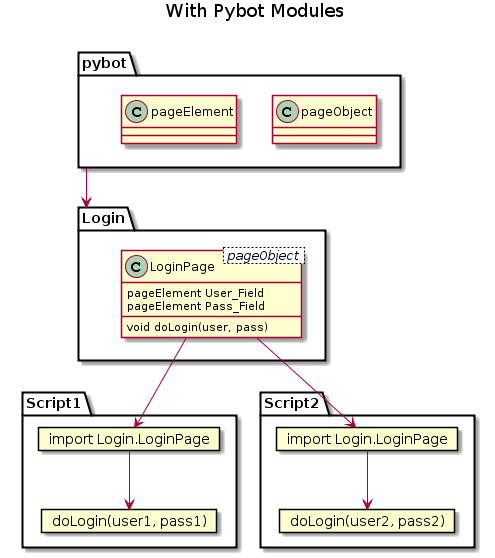
\includegraphics[width=0.8\textwidth]{./04-figuras/page_object_pybot}
        \label{fig:pybot_module}
    \end{figure}               % Uso do projeto


    % Elementos pós textuais
    \postextual
    %
% Documento: Referências Bibliográficas
%

\bibliography{refbase}    % Geração automática das referências por meio do arquivo 'refbase.bib'
       % Referências
    %
% Documento: Apêndices
%

\begin{apendicesenv}

    \chapter{Pesquisa de satisfação do Pybot}
    \label{app:quest}

    \begin{table}[H]
    \setlength\extrarowheight{25pt}
    \begin{tabular}{lccccc}
        Profissão:                    & (  )         & \multicolumn{1}{l}{Desenvolvedor}  & (  )         & \multicolumn{1}{l}{Testador}   &              \\
        Facilidade de Instalação:     & 1 $\bigcirc$ & 2 $\bigcirc$                       & 3 $\bigcirc$ & 4 $\bigcirc$                   & 5 $\bigcirc$ \\
        Facilidade de Uso:            & 1 $\bigcirc$ & 2 $\bigcirc$                       & 3 $\bigcirc$ & 4 $\bigcirc$                   & 5 $\bigcirc$ \\
        Atende necessidades básicas:  & 1 $\bigcirc$ & 2 $\bigcirc$                       & 3 $\bigcirc$ & 4 $\bigcirc$                   & 5 $\bigcirc$ \\
        Atende necessidades avançadas & 1 $\bigcirc$ & 2 $\bigcirc$                       & 3 $\bigcirc$ & 4 $\bigcirc$                   & 5 $\bigcirc$ \\
        Comentarios:                  & \multicolumn{5}{l}{\_\_\_\_\_\_\_\_\_\_\_\_\_\_\_\_\_\_\_\_\_\_\_\_\_\_\_\_\_}
    \end{tabular}
    \end{table}

    \chapter{Diagramas de Cenários}
    \label{app:imgs}

    \begin{figure}[H]
        \vspace*{0,3cm}
        \centering
        \caption{Uso padrão Selenium}
        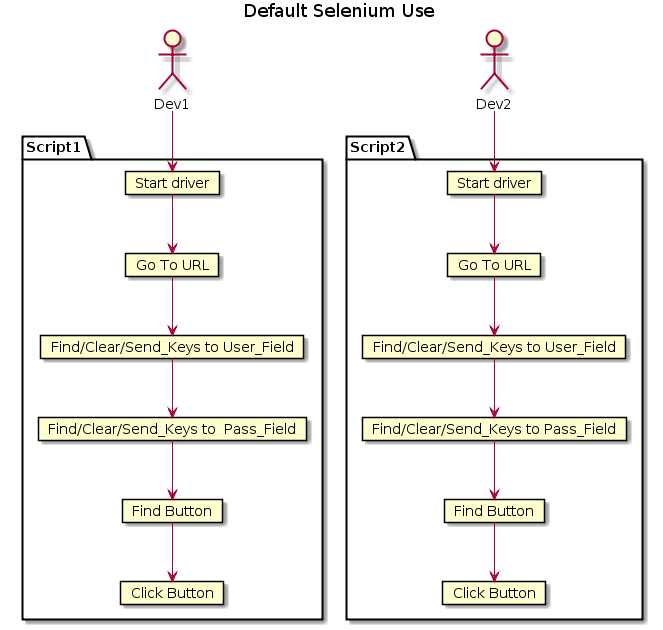
\includegraphics[width=1\textwidth]{./04-figuras/page_object_selenium}
        \label{fig:selenium_default}
    \end{figure}

    \begin{figure}[H]
        \vspace*{0,3cm}
        \centering
        \caption{Uso padrão Selenium com módulo}
        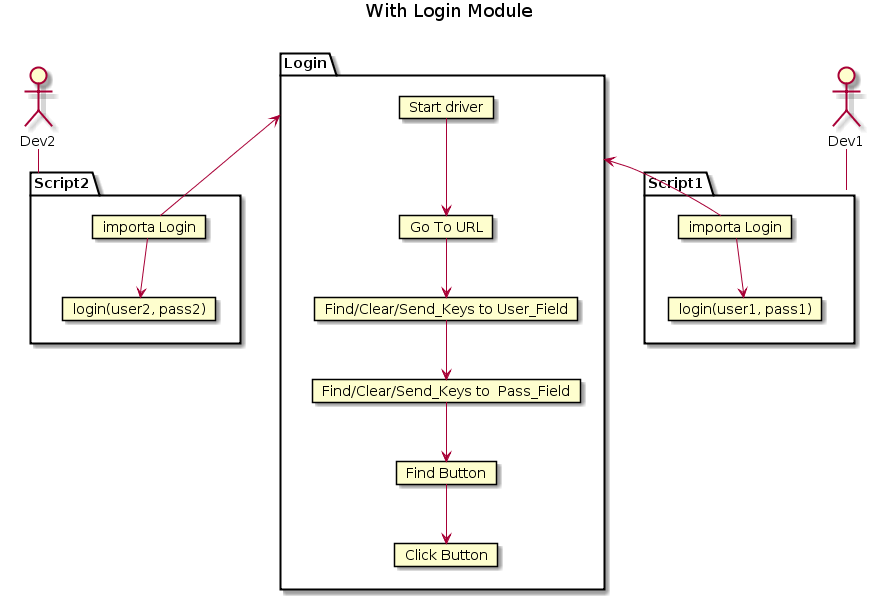
\includegraphics[width=1\textwidth]{./04-figuras/page_object_module}
        \label{fig:selenium_module}
    \end{figure}

    \begin{figure}[H]
        \vspace*{0,3cm}
        \centering
        \caption{Uso padrão Pybot}
        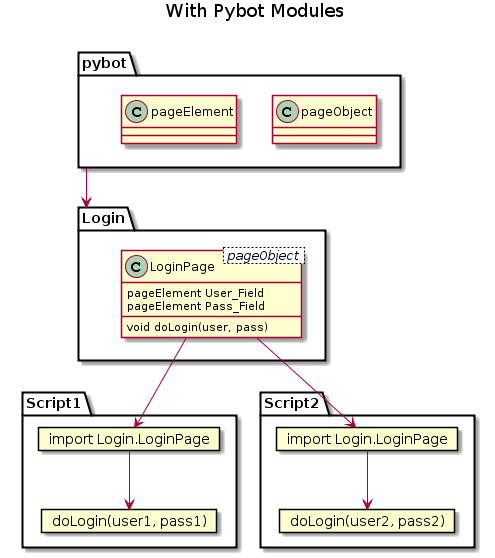
\includegraphics[width=1\textwidth]{./04-figuras/page_object_pybot}
        \label{fig:pybot_module}
    \end{figure}

\end{apendicesenv}         % Apêndices
    %
% Documento: Anexos
%

\begin{anexosenv}

\chapter{Como elaborar}

Anexo é texto ou documento não elaborado pelo autor, que serve de fundamentação, comprovação e ilustração. Elemento opcional. Deve ser precedido da palavra ANEXO, identifi-cado por letras maiúsculas consecutivas, travessão e pelo respectivo título. Utilizam-se letras maiúsculas dobradas, na identificação dos anexos, quando esgotadas as letras do alfabeto.


\end{anexosenv}            % Anexos
    %\printindex                                             % Índice remissivo

\end{document}
